% Root file used ashow macros
\documentclass{beamer}
\usepackage{tikz}
\usetikzlibrary{calc,arrows.meta,patterns}
\usepackage{xcolor}
\usepackage{multicol}
\usepackage{amsmath}
\usepackage{amssymb}
\hypersetup{colorlinks=true, linkcolor=blue}

% ================================================================
% Answer-overlay helpers
% ================================================================
\newcommand{\ablank}[1]{%
  \alt<2>{\textcolor{red}{\underline{#1}}}{\underline{\phantom{#1}}}%
}
\newcommand{\ashow}[1]{\uncover<2->{\textcolor{red}{\small #1}}}
\newcommand{\ashowq}[1]{\alt<2->{\textcolor{red}{\small #1}}{?}}

\title{Worked Solutions --- Circles: Parts, Perimeter \& Pi}
\author{}
\date{}

\begin{document}

\frame{\titlepage}

%------------------------------------------------
% CONTENTS
%------------------------------------------------
\begin{frame}{Contents}
  \framesubtitle{Click a link to jump to the first worked solution for that starter slide.}
  \begin{itemize}
    \item \hyperlink{s1q1}{Starter 1: Arithmetic, Lengths \& Decimals --- worked solutions}
    \item \hyperlink{s2q1}{Starter 2: Radius, Diameter \& Chord --- worked solutions}
    \item \hyperlink{s3q1}{Starter 3: Segments, Sectors, Arcs \& Tangents --- worked solutions}
    \item \hyperlink{s4q1}{Starter 4: Labelling, Pi \& Diameter --- worked solutions}
  \end{itemize}
  \medskip
  \begin{itemize}
    \item \hyperlink{questions1}{Starter 1: Questions \& short answers}
    \item \hyperlink{questions2}{Starter 2: Questions \& short answers}
    \item \hyperlink{questions3}{Starter 3: Questions \& short answers}
    \item \hyperlink{questions4}{Starter 4: Questions \& short answers}
  \end{itemize}
\end{frame}

%------------------------------------------------
% QUESTION COPY: STARTER 1
%------------------------------------------------
\begin{frame}[label=questions1]{Starter 1 --- Questions \& Short Answers}
\hypertarget{questions1}{}

\begin{columns}

\column{0.3\textwidth}
\begin{center}
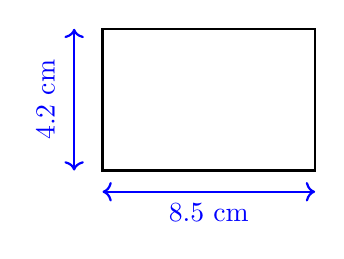
\begin{tikzpicture}[scale=0.9]
  % Rectangle for perimeter
  \draw[thick] (0,0) rectangle (3,2);
  \draw[blue, thick, <->] (0,-0.3) -- (3,-0.3);
  \node[blue] at (1.5,-0.6) {$8.5$ cm};
  \draw[blue, thick, <->] (-0.4,0) -- (-0.4,2);
  \node[blue, rotate=90] at (-0.8,1) {$4.2$ cm};
  
\end{tikzpicture}
\end{center}

\column{0.7\textwidth}
\small
\begin{enumerate}
    \begin{multicols}{2}
        \item $13 + 9 =$ \ashowq{$22$}
        \item $5.8 - 1.9 =$ \ashowq{$3.9$}
    \end{multicols}
    \begin{multicols}{2}
        \item $6 \times 8 =$ \ashowq{$48$}
        \item $4 \times 3.5$ \ashowq{$14$}
    \end{multicols}
  \item Round $3.14159$ to 2 decimal places. \ashow{$3.14$}
  \item A pencil is $12.8$ cm long. How many millimetres is this? \ablank{$128$ mm}
\end{enumerate}

\begin{enumerate}
  \setcounter{enumi}{4}
  \item Find the perimeter of the rectangle shown. \ashow{$25.4$ cm}
  \item The perimeter of a square is $26$ cm. What is the length of one side? \ashow{$6.5$ cm}
  \item  The perimeter of an equilateral triangle is $12.9$ cm. 
    Find the length of one side, and then the perimeter of a regular hexagon with the same side length. \ashow{$4.3$ cm; hexagon: $25.8$ cm}
\end{enumerate}

\end{columns}
\end{frame}

%------------------------------------------------
% QUESTION COPY: STARTER 2
%------------------------------------------------
\begin{frame}[label=questions2]{Starter 2 --- Questions \& Short Answers}
\hypertarget{questions2}{}

\begin{columns}

\column{0.3\textwidth}
\begin{center}
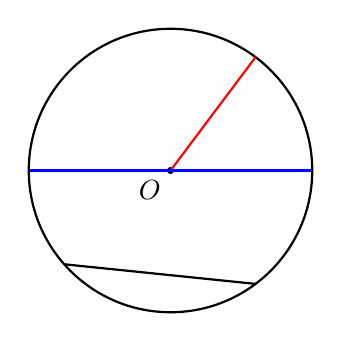
\begin{tikzpicture}[scale=0.9]
  % Circle
  \draw[thick] (0,0) circle (2cm);
  
  % Center
  \fill (0,0) circle (0.05);
  \node[below left] at (0,0) {$O$};
  
  % Radius
  \draw[red, thick] (0,0) -- (1.2,1.6);
  
  % Diameter
  \draw[blue, thick] (-2,0) -- (2,0);
  
  % Chord (not through center)
  \draw[thick] (-1.5,-1.323) -- (1.2,-1.6);

  
\end{tikzpicture}
\end{center}

\column{0.7\textwidth}
\small
\begin{enumerate}
\begin{multicols}{2}
  \item $24 \div 6$ \ashow{$=4$}
  \item $72 \div 8$ \ashow{$=9$}
  \end{multicols}
  \begin{multicols}{2}
  \item Double $15.5$ \ashow{$=31$}
  \item Halve $31.4$ \ashow{$=15.7$}
  \end{multicols}
  \item How many centimetres in $1.2$ metres? \ashow{$120$ cm}
  \item True or false? $2.5 \times 4 = 10$ \ashow{True}
\end{enumerate}

\begin{enumerate}
  \setcounter{enumi}{4}
  \item On the diagram, which line is the \textbf{diameter}? 
    How is it different from a chord? \ashow{Blue line; a diameter passes through the centre.}
  \item If the radius of a circle is $7$ cm, what is its diameter? \ashow{$14$ cm}
  \item The diameter of a circle is $18$ mm. Find its radius. \ablank{$9$ mm}
  \item A chord of length $8$ cm is drawn inside a circle of radius $5$ cm.
    Is the chord a diameter? Explain. \ashow{No; a diameter would be $10$ cm.}
\end{enumerate}

\end{columns}
\end{frame}

%------------------------------------------------
% QUESTION COPY: STARTER 3
%------------------------------------------------
\begin{frame}[label=questions3]{Starter 3 --- Questions \& Short Answers}
\hypertarget{questions3}{}

\begin{columns}

\column{0.35\textwidth}

\begin{center}
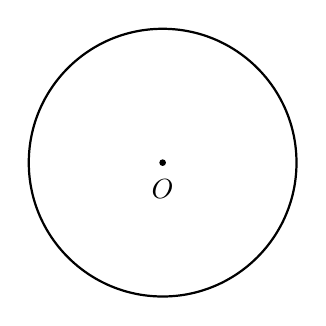
\begin{tikzpicture}[scale=0.85]
  % Circle
  \draw[thick] (0,0) circle (2cm);
  \fill (0,0) circle (0.05);
  \node[below] at (0,-0.1) {$O$};

\end{tikzpicture}

\vspace{3em}

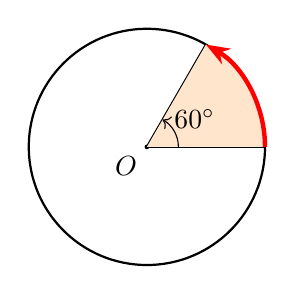
\begin{tikzpicture}[scale=1]
  % Circle
  \draw[thick] (0,0) circle (1.5cm);
  
  % Centre
  \fill (0,0) circle (0.03);
  \node[below left] at (0,0) {$O$};
  
  % Radii that bound the 60° sector
  \draw[thick] (0,0) -- (0:1.5);          % right horizontal radius
  \draw[thick] (0,0) -- (60:1.5);         % radius at 60°
  

  
  % Optional: shade the sector lightly
  \fill[orange!20] (0,0) -- (0:1.5) arc (0:60:1.5) -- cycle;

    % Highlight the arc (thick, coloured, with arrow)
  \draw[red, ultra thick, -{Stealth[length=3mm]}] 
    (0:1.5) arc (0:60:1.5);
  
  % Angle arc and label
  \draw[->] (0.4,0) arc (0:60:0.4);
  \node at (30:0.7) {$60^\circ$};
  
\end{tikzpicture}

\end{center}


\column{0.65\textwidth}
\small
\begin{enumerate}
\begin{multicols}{2}
  \item $3.2 \times 5$ \ashow{$=16$}
  \item $1.8 \times 4$ \ashow{$=7.2$}
  \end{multicols}
  \begin{multicols}{2}
    \item  $45 \div 10$ \ashow{$=4.5$}
    \item $90 \div 100$ \ashow{$=0.9$}
  \end{multicols}
  \item What is $\frac{1}{4}$ of $360^\circ$? \ashow{$90^\circ$}
\end{enumerate}

\begin{enumerate}
  \setcounter{enumi}{5}
  \item Copy the diagram, and draw with labels:
    \begin{multicols}{2}
    \begin{itemize}
      \item A sector
      \item An arc
      \item A tangent
      \item A segment
    \end{itemize}
    \end{multicols}
    \ashow{Sector: shaded slice; Arc: curved boundary; Tangent: line touching the circle once; Segment: region between a chord and an arc.}
  \item If the radius is $6$ cm, what is the whole circumference? (Use $\pi \approx 3.14$) \ashow{$37.68$ cm}
  \item For the sector shown, what fraction of the circumference is the arc length? Calculate the arc length if the whole circle has a circumference of 24cm. \ashow{$\frac{1}{6}$; $4$ cm}

\end{enumerate}

\end{columns}
\end{frame}

%------------------------------------------------
% QUESTION COPY: STARTER 4
%------------------------------------------------
\begin{frame}[label=questions4]{Starter 4 --- Questions \& Short Answers}
\hypertarget{questions4}{}

\vspace{-2em}

\begin{columns}

\column{0.3\textwidth}
\begin{center}
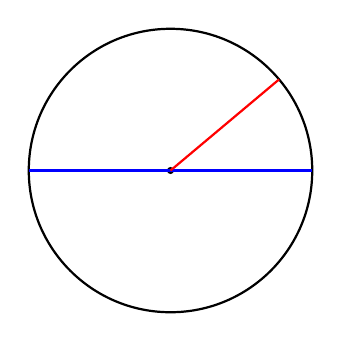
\begin{tikzpicture}[scale=0.9]
  % Circle with labels
  \draw[thick] (0,0) circle (2cm);
  \fill (0,0) circle (0.05);
  
  \draw[blue, thick] (-2,0) -- (2,0);
  
  \draw[red, thick] (0,0) -- (40:2);
  
\end{tikzpicture}

\end{center}

\column{0.7\textwidth}
\small
\begin{enumerate}
\begin{multicols}{2}
  \item $12 \times 3 $ \ashow{$=36$}
  \item $4 \times 3.14$ \ashow{$=12.56$}
\end{multicols}
\begin{multicols}{2}
  \item $6.28 \div 2 $ \ashow{$=3.14$} 
  \item $ 9.42 \div 3$ \ashow{$=3.14$}
  \end{multicols}
  \item Round $3.14159265$ to 3 decimal places. \ashow{$3.142$}
  \begin{multicols}{2}
  \item Double $3.14$ \ashow{$=6.28$}
  \item halve $12.56$ \ashow{$=6.28$}
  \end{multicols}
\end{enumerate}
\vspace{-0.5em}
\begin{enumerate}
  \setcounter{enumi}{7}
  \item Copy and label on the diagram: 
    centre, radius, diameter, circumference. \ashow{centre: $O$; radius: red line; diameter: blue line; circumference: the circle itself}
    \item Draw a chord on the diagram shorter than the radius \ashow{Many possible answers, e.g.\ a chord close to the circumference}
    \item Draw a chord on the diagram longer than the radius \ashow{Many possible answers, e.g.\ a chord passing near the centre but not through it}
  
  \item If the diameter is $8$ cm, what is:
    \begin{itemize}
      \item the radius? \ashow{$4$ cm}
      \item the circumference? ($\pi \approx 3.14$) \ashow{$25.12$ cm}
    \end{itemize}
 
\end{enumerate}

\end{columns}
\end{frame}

%------------------------------------------------
% WORKED SOLUTIONS: STARTER 1
%------------------------------------------------
\begin{frame}[label=s1q1]{Starter 1, Q1}
\hypertarget{s1q1}{}
$13+9$: split into $10+3+9=10+12=22$.
\ashow{Answer: $22$}
\end{frame}

\begin{frame}[label=s1q2]{Starter 1, Q2}
\hypertarget{s1q2}{}
$5.8-1.9$: subtract $1.8$ first:
\[
5.8-1.8=4.0
\]
Then subtract the remaining $0.1$:
\[
4.0-0.1=3.9
\]
\ashow{Answer: $3.9$}
\end{frame}

\begin{frame}[label=s1q3]{Starter 1, Q3}
\hypertarget{s1q3}{}
\[
6\times 8 = 48
\]
\ashow{Answer: $48$}
\end{frame}

\begin{frame}[label=s1q4]{Starter 1, Q4}
\hypertarget{s1q4}{}
$4\times 3.5$: double $3.5$ twice.
\[
3.5\times 2 = 7, \qquad 7\times 2 = 14
\]
\ashow{Answer: $14$}
\end{frame}

\begin{frame}[label=s1q5]{Starter 1, Q5}
\hypertarget{s1q5}{}
Round $3.14159$ to 2 decimal places.
The third decimal digit is $1$, which is less than $5$, so the second decimal digit stays as $4$.
\[
3.14159 \approx 3.14
\]
\ashow{Answer: $3.14$}
\end{frame}

\begin{frame}[label=s1q6]{Starter 1, Q6}
\hypertarget{s1q6}{}
$1$ cm $=10$ mm, so multiply by $10$.
\[
12.8 \times 10 = 128
\]
\ashow{Answer: $128$ mm}
\end{frame}

\begin{frame}[label=s1q7]{Starter 1, Q7}
\hypertarget{s1q7}{}
Perimeter of a rectangle:
\[
P=2(\text{length}+\text{width})
=2(8.5+4.2)
=2(12.7)
=25.4
\]
\ashow{Answer: $25.4$ cm}
\end{frame}

\begin{frame}[label=s1q8]{Starter 1, Q8}
\hypertarget{s1q8}{}
A square has four equal sides.
\[
\text{side length}=\frac{26}{4}=6.5
\]
\ashow{Answer: $6.5$ cm}
\end{frame}

\begin{frame}[label=s1q9]{Starter 1, Q9}
\hypertarget{s1q9}{}
An equilateral triangle has three equal sides.
\[
\text{one side}=\frac{12.9}{3}=4.3
\]
A regular hexagon has six equal sides, so its perimeter is:
\[
6\times 4.3=25.8
\]
\ashow{Answer: $4.3$ cm; hexagon: $25.8$ cm}
\end{frame}

%------------------------------------------------
% WORKED SOLUTIONS: STARTER 2
%------------------------------------------------
\begin{frame}[label=s2q1]{Starter 2, Q1}
\hypertarget{s2q1}{}
\[
24\div 6 = 4
\]
\ashow{Answer: $4$}
\end{frame}

\begin{frame}[label=s2q2]{Starter 2, Q2}
\hypertarget{s2q2}{}
\[
72\div 8 = 9
\]
\ashow{Answer: $9$}
\end{frame}

\begin{frame}[label=s2q3]{Starter 2, Q3}
\hypertarget{s2q3}{}
Double $15.5$ means multiply by $2$.
\[
15.5\times 2 = 31
\]
\ashow{Answer: $31$}
\end{frame}

\begin{frame}[label=s2q4]{Starter 2, Q4}
\hypertarget{s2q4}{}
Halve $31.4$ means divide by $2$.
\[
31.4\div 2 = 15.7
\]
\ashow{Answer: $15.7$}
\end{frame}

\begin{frame}[label=s2q5]{Starter 2, Q5}
\hypertarget{s2q5}{}
$1$ m $=100$ cm, so multiply by $100$.
\[
1.2\times 100 = 120
\]
\ashow{Answer: $120$ cm}
\end{frame}

\begin{frame}[label=s2q6]{Starter 2, Q6}
\hypertarget{s2q6}{}
\[
2.5\times 4 = 10
\]
So the statement is true.
\ashow{Answer: True}
\end{frame}

\begin{frame}[label=s2q7]{Starter 2, Q7}
\hypertarget{s2q7}{}
The blue line passes through the centre $O$, so it is the diameter.
A chord is any line segment joining two points on the circumference.
A diameter is a special chord that passes through the centre.
\ashow{Answer: Blue line; a diameter passes through the centre.}
\end{frame}

\begin{frame}[label=s2q8]{Starter 2, Q8}
\hypertarget{s2q8}{}
\[
\text{diameter}=2\times \text{radius}=2\times 7=14
\]
\ashow{Answer: $14$ cm}
\end{frame}

\begin{frame}[label=s2q9]{Starter 2, Q9}
\hypertarget{s2q9}{}
\[
\text{radius}=\frac{\text{diameter}}{2}=\frac{18}{2}=9
\]
\ashow{Answer: $9$ mm}
\end{frame}

\begin{frame}[label=s2q10]{Starter 2, Q10}
\hypertarget{s2q10}{}
A diameter of this circle would be:
\[
2\times 5=10\text{ cm}
\]
The given chord is only $8$ cm long, so it is not a diameter.
\ashow{Answer: No; a diameter would be $10$ cm.}
\end{frame}

%------------------------------------------------
% WORKED SOLUTIONS: STARTER 3
%------------------------------------------------
\begin{frame}[label=s3q1]{Starter 3, Q1}
\hypertarget{s3q1}{}
\[
3.2\times 5 = 16
\]
\ashow{Answer: $16$}
\end{frame}

\begin{frame}[label=s3q2]{Starter 3, Q2}
\hypertarget{s3q2}{}
\[
1.8\times 4 = 7.2
\]
\ashow{Answer: $7.2$}
\end{frame}

\begin{frame}[label=s3q3]{Starter 3, Q3}
\hypertarget{s3q3}{}
\[
45\div 10 = 4.5
\]
\ashow{Answer: $4.5$}
\end{frame}

\begin{frame}[label=s3q4]{Starter 3, Q4}
\hypertarget{s3q4}{}
\[
90\div 100 = 0.9
\]
\ashow{Answer: $0.9$}
\end{frame}

\begin{frame}[label=s3q5]{Starter 3, Q5}
\hypertarget{s3q5}{}
\[
\frac{1}{4}\text{ of }360^\circ = 360^\circ\div 4 = 90^\circ
\]
\ashow{Answer: $90^\circ$}
\end{frame}

\begin{frame}[label=s3q6]{Starter 3, Q6}
\hypertarget{s3q6}{}
A \textbf{sector} is the region bounded by two radii and the arc between them.  
An \textbf{arc} is part of the circumference.  
A \textbf{tangent} is a straight line that touches the circle at exactly one point.  
A \textbf{segment} is the region between a chord and the arc cut off by the chord.
\ashow{Answer: Sector: shaded slice; Arc: curved boundary; Tangent: line touching the circle once; Segment: region between a chord and an arc.}
\end{frame}

\begin{frame}[label=s3q7]{Starter 3, Q7}
\hypertarget{s3q7}{}
\[
C=2\pi r = 2\times 3.14\times 6
\]
First:
\[
2\times 3.14=6.28
\]
Then:
\[
6.28\times 6 = 37.68
\]
\ashow{Answer: $37.68$ cm}
\end{frame}

\begin{frame}[label=s3q8]{Starter 3, Q8}
\hypertarget{s3q8}{}
The sector angle is $60^\circ$, so the arc is:
\[
\frac{60}{360}=\frac{1}{6}
\]
of the circumference.
\[
\text{arc length}=\frac{1}{6}\times 24 = 4
\]
\ashow{Answer: $\frac{1}{6}$; $4$ cm}
\end{frame}

%------------------------------------------------
% WORKED SOLUTIONS: STARTER 4
%------------------------------------------------
\begin{frame}[label=s4q1]{Starter 4, Q1}
\hypertarget{s4q1}{}
\[
12\times 3 = 36
\]
\ashow{Answer: $36$}
\end{frame}

\begin{frame}[label=s4q2]{Starter 4, Q2}
\hypertarget{s4q2}{}
\[
4\times 3.14 = 12.56
\]
\ashow{Answer: $12.56$}
\end{frame}

\begin{frame}[label=s4q3]{Starter 4, Q3}
\hypertarget{s4q3}{}
\[
6.28\div 2 = 3.14
\]
\ashow{Answer: $3.14$}
\end{frame}

\begin{frame}[label=s4q4]{Starter 4, Q4}
\hypertarget{s4q4}{}
\[
9.42\div 3 = 3.14
\]
\ashow{Answer: $3.14$}
\end{frame}

\begin{frame}[label=s4q5]{Starter 4, Q5}
\hypertarget{s4q5}{}
Round $3.14159265$ to 3 decimal places.
The fourth decimal digit is $5$, so round the third decimal digit up from $1$ to $2$.
\[
3.14159265 \approx 3.142
\]
\ashow{Answer: $3.142$}
\end{frame}

\begin{frame}[label=s4q6]{Starter 4, Q6}
\hypertarget{s4q6}{}
\[
\text{double }3.14 = 2\times 3.14 = 6.28
\]
\ashow{Answer: $6.28$}
\end{frame}

\begin{frame}[label=s4q7]{Starter 4, Q7}
\hypertarget{s4q7}{}
\[
\text{halve }12.56 = 12.56\div 2 = 6.28
\]
\ashow{Answer: $6.28$}
\end{frame}

\begin{frame}[label=s4q8]{Starter 4, Q8}
\hypertarget{s4q8}{}
Centre: point $O$.  
Radius: the red line from $O$ to the circumference.  
Diameter: the blue line through $O$, from one side of the circle to the other.  
Circumference: the circle boundary itself.
\ashow{Answer: centre $O$; radius red line; diameter blue line; circumference the circle itself.}
\end{frame}

\begin{frame}[label=s4q9]{Starter 4, Q9}
\hypertarget{s4q9}{}
A chord shorter than the radius should be drawn close to the circumference, so its length is small.  
For example, in a circle of radius $2$ cm, a chord of length $1.5$ cm is shorter than the radius.
\ashow{Answer: Many possible answers, e.g.\ a chord close to the circumference.}
\end{frame}

\begin{frame}[label=s4q10]{Starter 4, Q10}
\hypertarget{s4q10}{}
A chord longer than the radius can be drawn near the centre, but not through the centre.  
For example, in a circle of radius $2$ cm, a chord of length $3$ cm is longer than the radius.
\ashow{Answer: Many possible answers, e.g.\ a chord passing near the centre but not through it.}
\end{frame}

\begin{frame}[label=s4q11]{Starter 4, Q11}
\hypertarget{s4q11}{}
\[
\text{radius}=\frac{\text{diameter}}{2}=\frac{8}{2}=4
\]
\[
\text{circumference}=\pi d = 3.14\times 8 = 25.12
\]
\ashow{Answer: radius $4$ cm; circumference $25.12$ cm}
\end{frame}

\end{document}